\documentclass[24 pts]{article}
\usepackage{xeCJK}
\usepackage{amssymb}
\usepackage{amsmath}
\usepackage{amsthm}
\usepackage{graphicx}
\graphicspath{ {images/} }
\usepackage{relsize}

\newcommand{\me}{\mathrm{e}}
\setCJKmainfont[BoldFont= Yu Mincho Demibold]{MS Mincho}
\title{Advanced Radio Communication Engineering Report -Professor T. Kojima }
\date{June 15 2016}
\author{Kwame Ackah Bohulu 1631133}
\begin{document}
\maketitle
[1]BER for equal energy binary transmission system based on ML criteria is given as 
\begin{equation*}
P_b = \frac{1}{2}erfc\sqrt{\frac{(1-\rho)E_b}{2N_0}}\\
\end{equation*}
where
\begin{equation*}
\rho =\frac{1}{E_b}\int_{-\infty}^{\infty}s_0(t) s_1(t)dt
\end{equation*}
since the signals have equal energy 
$$\int_{-\infty}^{\infty}s_0(t) ^2dt=\int_{-\infty}^{\infty}s_1(t) ^2dt=E_b$$

$s_0(t),s_1(t),s_0(t)s_1(t)$ are defined below
\[
s_0(t)=
\begin{cases}
1&,(0\leq t<T/2)\\
-1&,(T/2\leq t<T)\\
0,&(otherwise)
 \end{cases}
\]

\[
s_1(t)=
\begin{cases}
-1&,(0\leq t<7T/20)\\
1&,(7T/20\leq t<T)\\
0,&(otherwise)
 \end{cases}
\]

\[
s_0(t)s_1(t)=
\begin{cases}
-1&,(0\leq t<7T/20)\\
1&,(7T/20\leq t<T/2)\\
-1&,(T/2\leq t<T)\\
0,&(otherwise)
 \end{cases}
\]
therefore
$$E_b=\int_{0}^{T}s_0(t) ^2=T$$
and
$$\rho=\frac{1}{T}\left[\,-\int_{0}^{7T/20}dt+\int_{7T/20}^{T/2}dt-\int_{T/2}^{T}dt\right]\,=\frac{-7}{10}$$
substituting the value of $\rho$ and $E_b$ into the BER equation gives
$$P_b = \frac{1}{2}erfc\sqrt{\frac{(1+7/10)T}{2N_0}} =\frac{1}{2}erfc\sqrt{\frac{17T}{20N_0}}$$ 
\paragraph{}
[2]The figure below shows the constellation diagrams for 16QAM and 16PSK.
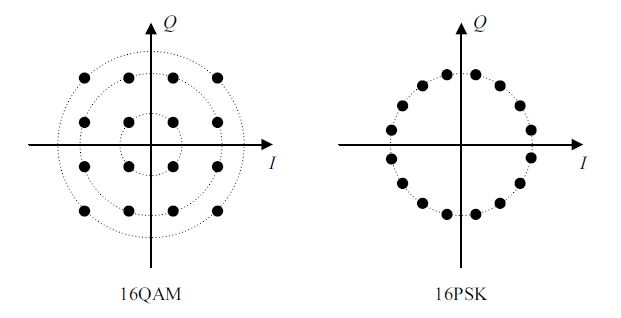
\includegraphics[scale =0.5]{Capture}\\
 Assuming minimum Euclidean distance is the same, it is denoted by $d_{min}$.
the radius for the various circles in the 16QAM constellation are defined below
\begin{equation*}
\begin{split}
circle 1 \, \,\,\,\,\,\,&\frac{\sqrt{2}}{2}d_{min}\\
circle \,2  \,\,\,\,\,\,\, &\frac{\sqrt{10}}{2}d_{min}\\
 circle \,3 \,\,\,\,\,\,\, &\frac{3\sqrt{2}}{2}d_{min}
\end{split}
\end{equation*}
therefore, the Energy per symbol for 16QAM, $E_s$ is given below
$$E_s=\frac{1}{16}\left(\,4\cdot \frac{\sqrt{2}}{2}d_{min}^2+8\cdot \frac{\sqrt{10}}{2}d_{min}^2+4\cdot \frac{3\sqrt{2}}{2}d_{min}^2\right)\,=\frac{5}{2}d_{min}^2$$
For the case of 16PSK the radius of the circle is given by
$$\frac{d_{min}}{2\sin( \pi/16)}$$
therefore, the Energy per symbol for 16PSK, $E_s^{'}$ is given below
$$E_s^{'}=\frac{d_{min}^2}{4\sin^2( \pi/16)}$$
finally, $$\frac{E_s^{'}}{E_s}=\frac{1}{10\sin^2( \pi/16)}=2.6274$$






\end{document}